% ============================================================
% Results draft generated from the frozen analysis tables.
% Replace cross-references after final figure/table numbering is fixed.
% ============================================================

\subsection{Expression-guided selection of candidate SLRPs}
\label{subsec:results-expression}

The initial expression screen measured nine SLRP genes in three samples of
P0-derived Prx1-lineage chondrocyte material from NCBI GEO GSE305415. BGN had the
highest mean abundance (3012.762 TPM), followed by OGN (657.412 TPM), FMOD
(605.864 TPM), DCN (581.246 TPM), LUM (272.457 TPM), PRELP (189.840 TPM),
ASPN (112.954 TPM),
EPYC (99.059 TPM), and OMD (96.317 TPM). Because these samples represented a
P0-derived skeletal lineage rather than anatomically isolated growth-plate zones,
the screen was treated as a prioritization dataset and not as direct evidence
of growth-plate-specific expression. The deposited series and sample records
disagree about whether RNA was extracted before or after culture; therefore,
these values were not attributed to an exact in-vivo chondrocyte state.

Processed microdissected tibial growth-plate data from mouse and rat
(GSE114919) provided the direct anatomical comparison. BGN, FMOD, and PRELP
ranked consistently highly across the examined age-by-zone conditions. LUM and
EPYC showed intermediate support, whereas OGN ranked lower, particularly in
rat. The numerical scales of the GSE305415-derived TPM dataset and GSE114919
were not pooled. Bgee call summaries and gene-specific literature were used as
independent contextual evidence rather than as replacements for the two
expression analyses. Figure~\ref{fig:expression-evidence} presents these two
complementary expression layers without combining their numerical scales.

The final comparative panel therefore comprised BGN, DCN, FMOD, PRELP, EPYC,
LUM, and OGN. Selection was not based on abundance alone: the panel also represented
SLRP classes I--III, included genes with direct cartilage or skeletal evidence,
and retained OGN as an explicitly exploratory class-III member. DCN was included
as a full class-I candidate and the closest paralog control for BGN. OMD was
retained as a context gene because of its
skeletal literature and conserved representative gene structure, but it was not
advanced to the full protein, phylogeny, and synteny workflow. ASPN was retained
as class-I background rather than advanced to the seven-gene panel: it ranked
seventh in the P0-derived screen, its independent tibial growth-plate support
was weaker and inconsistent between mouse and rat, and BGN plus the DCN paralog
control already supplied the main class-I comparison. This was a scope and
evidence-prioritization decision, not a claim that ASPN is absent from cartilage.

\begin{figure}[htbp]
    \centering
    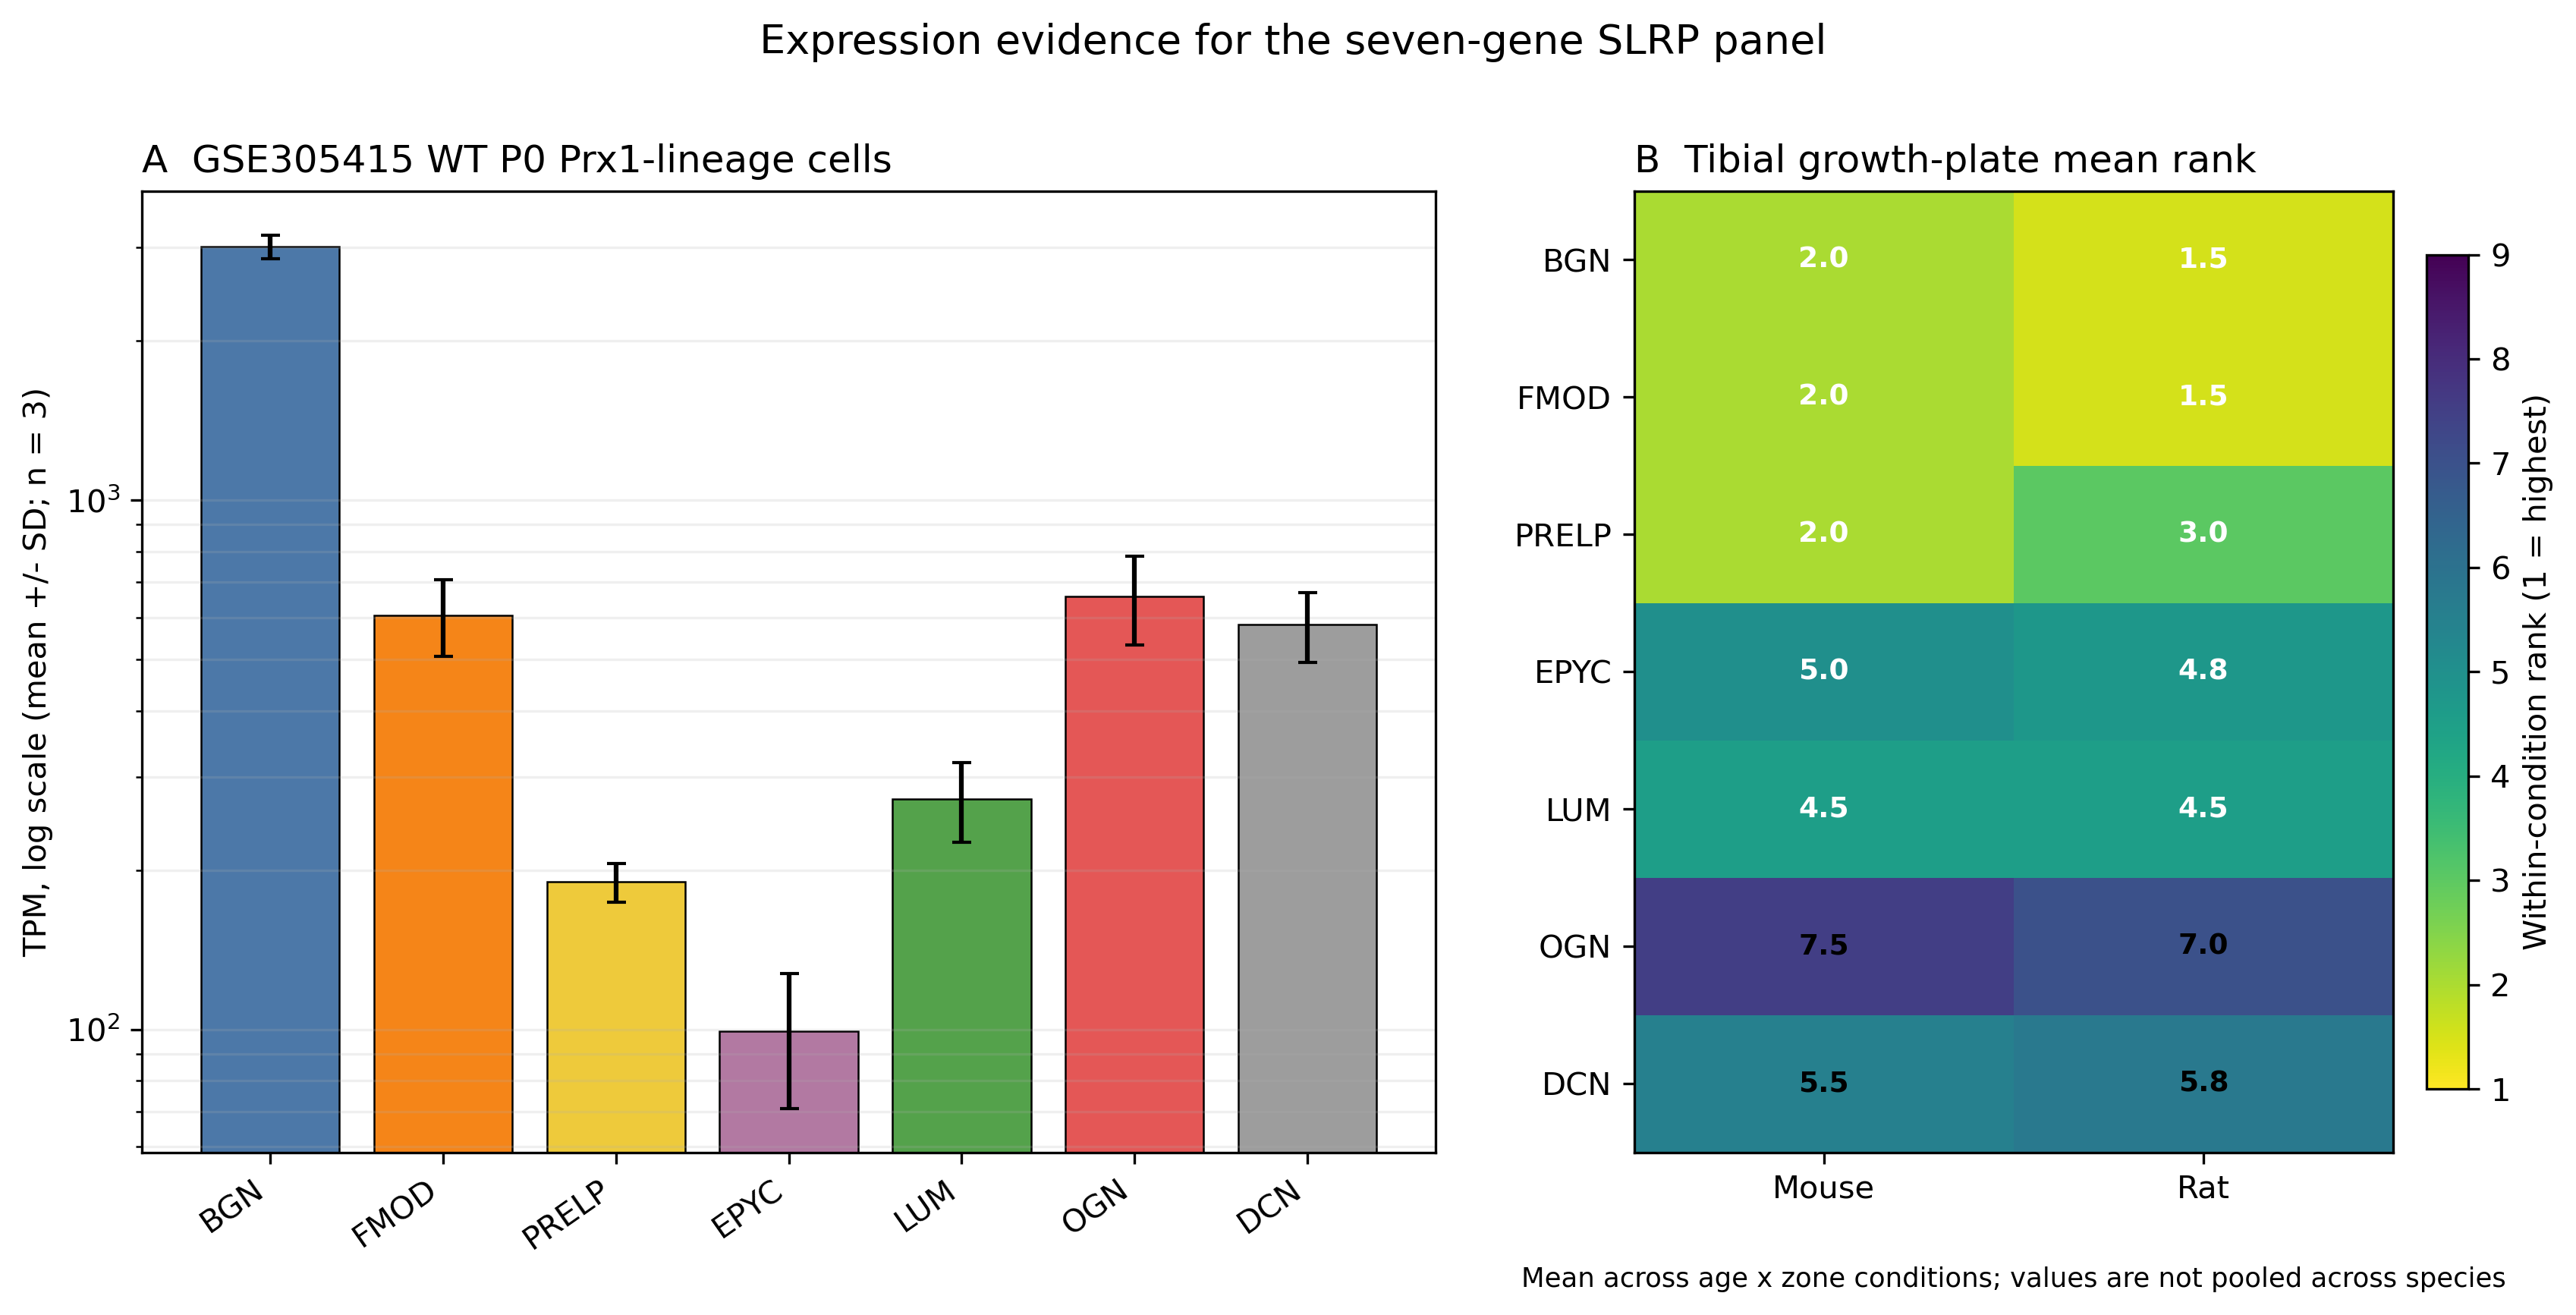
\includegraphics[width=\textwidth,height=0.76\textheight,keepaspectratio]
        {figures/expression/expression_evidence.png}
    \caption{Expression evidence used to prioritize the seven-gene SLRP panel.
    Panel A summarizes mean expression in three samples of P0-derived
    Prx1-lineage chondrocyte material from NCBI GEO GSE305415; error bars show
    standard deviation and the abundance axis is logarithmic. Panel B
    summarizes within-condition ranks in
    processed mouse and rat microdissected tibial growth-plate data
    (GSE114919). The two numerical scales were not pooled. Expression was used
    for biological prioritization and does not establish function or orthology.
    Because the deposited records conflict about culture before RNA extraction,
    the exact cell state is not assigned.}
    \label{fig:expression-evidence}
\end{figure}

\subsection{Cross-species candidate recovery and manual protein curation}
\label{subsec:results-protein-conservation}

After reciprocal-hit, annotation, length, and duplication checks, the confident
canonical panel contained 103 nonredundant proteins: BGN 13, DCN 15, FMOD 14,
PRELP 16, EPYC 15, LUM 16, and OGN 14. Four historical BGN assignments were
removed as DCN or DCN-like records, and tentative partial replacement models
were retained for catshark and whale shark. The amphioxus sequence
\texttt{XP\_066265713.1} was removed from the confident OGN ortholog set after
manual alignment review and disagreement among tree, synteny, and reciprocal-hit
evidence. It was retained only as an uncertain SLRP-like provenance record. The
chicken BGN-locus product \texttt{XP\_414298.2} was likewise excluded from the
canonical BGN protein set because its product annotation, reciprocal hit, and a
focused reference tree supported ASPN rather than BGN.

\subsubsection{Conserved domain architecture and alignment continuity}

Across the final panel, 102 of 103 proteins met the current SLRP/LRR-family
criterion. SignalP results were available for all 103 proteins: 100 were
positive and three were negative. The final 17-sequence run produced 15
positive calls; its negative calls were the fragmentary whale-shark BGN
\texttt{XP\_048475905.1} and opossum DCN \texttt{XP\_001363160.3}. The third
negative record was spotted-gar OGN \texttt{XP\_006631165.2}. Manual inspection
showed an intact OGN protein and a continuous LRR-rich alignment, so it was
retained as tentative while uncertainty about its N-terminal secretion signal
was recorded. The exact spotted-gar GFF contained only one \textit{ogna}
transcript (\texttt{XM\_006631102.3}), so no annotated alternative N terminus
could be substituted. Although residues 8--25 form a strongly hydrophobic
N-terminal segment, SignalP classified the sequence as OTHER (SP score 0.167)
without a cleavage call; this supported no confidence upgrade. Opossum OGN
\texttt{XP\_056660002.1} and zebrafish OGN \texttt{NP\_001013588.1} were
retained after manual inspection of termini, conserved cysteine positions, and
alignment continuity. The whale-shark EPYC sequence
\texttt{XP\_048463897.1} was retained as tentative. Manual inspection found a
similar early N-terminal beginning and a strongly conserved
middle-to-C-terminal region, but numerous mismatches in the earlier portion,
reduced query coverage, and an alternative reciprocal hit prevented an
unqualified assignment.

Focused review resolved the four outstanding class-I protein questions.
Catshark BGN \texttt{XP\_038638277.1} has a strong signal peptide, conserved
comparable cysteines and SLRP/LRR domains, but lacks approximately 111
human-equivalent C-terminal residues; it was retained as a tentative partial
ortholog. Whale-shark BGN \texttt{XP\_048475905.1} is a discontinuous 161-aa
fragment at a syntenically supported BGN locus and lacks a detectable signal
peptide; it was retained only as a tentative locus/fragment record and excluded
from complete-protein claims. Opossum DCN \texttt{XP\_001363160.3} is a highly
conserved C-terminal fragment that lacks the N-terminal signal-peptide region;
its protein assignment was retained, while its locus remained unresolved
because the SynVoy FASTA and GFF versions do not match. Catshark DCN
\texttt{XP\_038636759.1} spans the full aligned core, retains all six comparable
cysteines, lies in the DCN tree split and has a SignalP-positive N terminus. It
was retained confidently, with its 29-aa N-terminal extension and predicted
cleavage between residues 45 and 46 recorded as a gene-model caveat.

All seven gene-specific alignments retained a conserved core despite variation at
the termini and in gap-rich regions. Exact amino-acid identity was not required
for orthology: manual review emphasized intact termini, conserved cysteines,
continuous alignment through the LRR-rich region, absence of large
sequence-specific insertions or deletions, and agreement with independent tree,
synteny, and SignalP evidence. Figure~\ref{fig:protein-conservation} summarizes
the alignment, domain, signal-peptide, and candidate-level quality-control
evidence across the final 103-protein panel.

\begin{figure}[htbp]
    \centering
    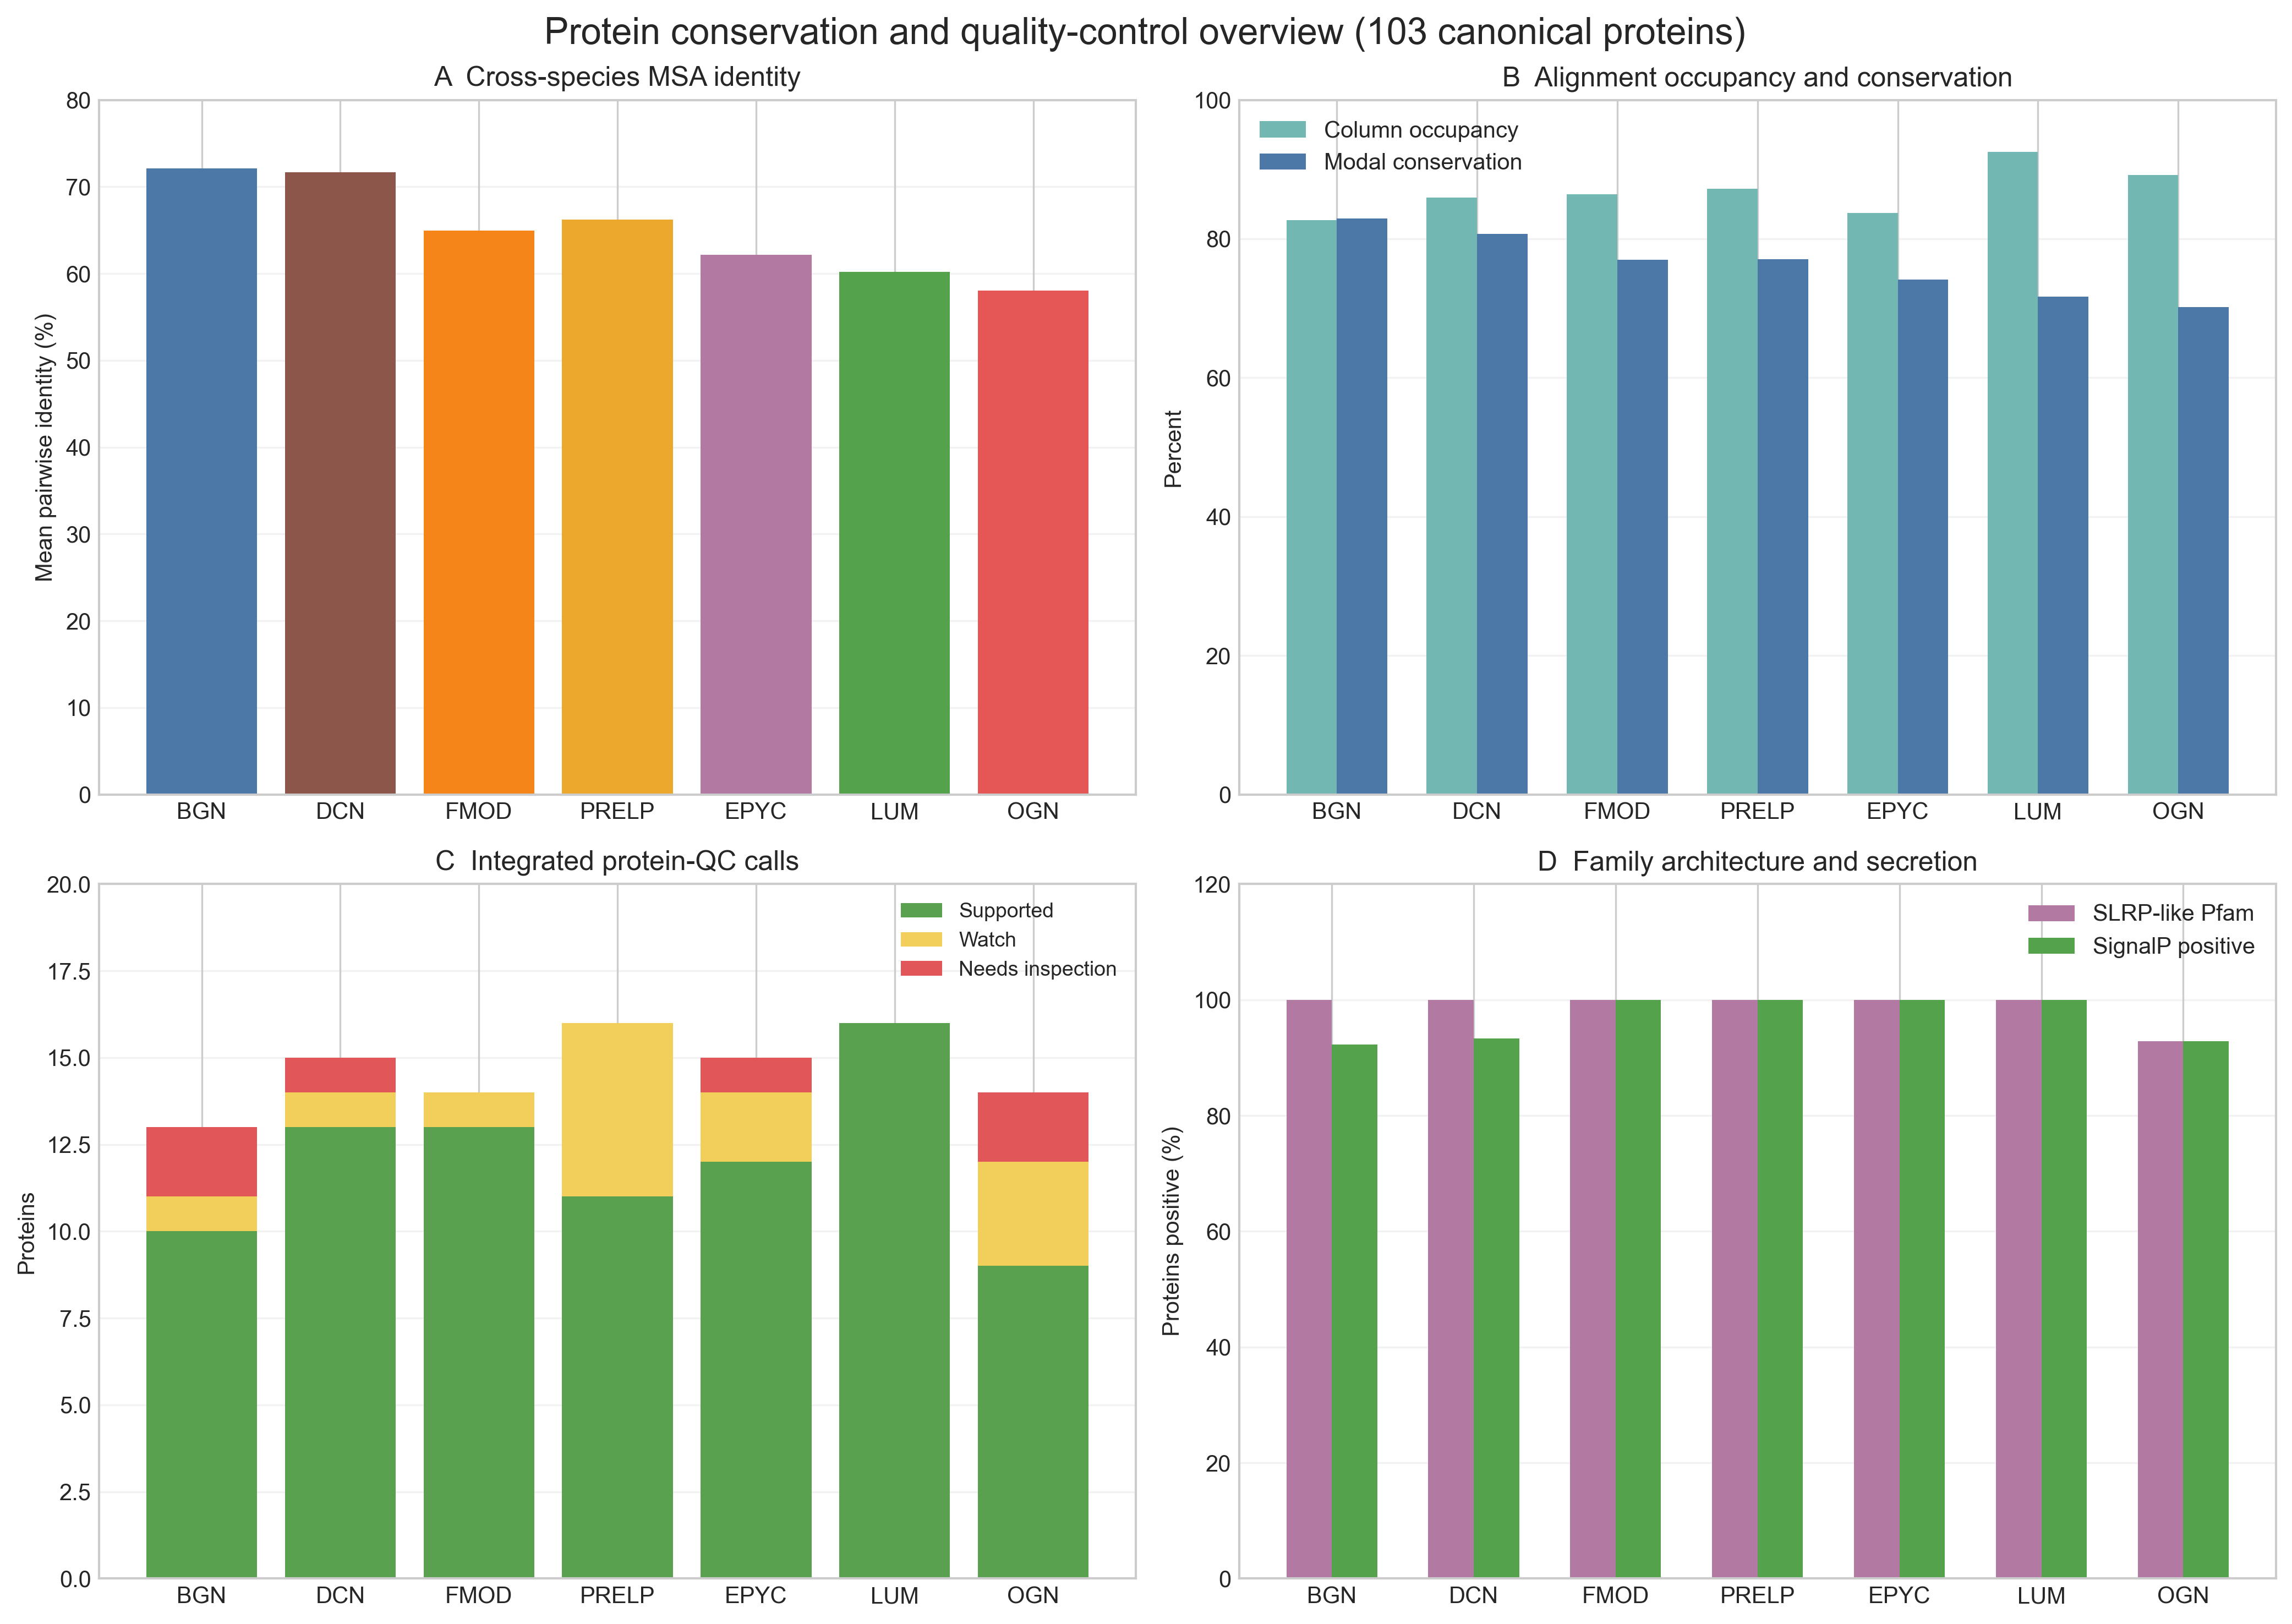
\includegraphics[width=\textwidth,height=0.76\textheight,keepaspectratio]
        {figures/protein/protein_conservation_overview.png}
    \caption{Protein conservation and quality-control summary for the
    103-protein canonical SLRP panel. The panels summarize within-gene sequence
    identity, alignment occupancy and modal-residue conservation, integrated
    candidate flags, Pfam SLRP/LRR-family support, and SignalP-positive calls.
    SignalP results are complete for all 103 proteins (100 positive and three
    negative). These measures
    support conserved secreted SLRP architecture but do not individually prove
    gene-specific orthology or conserved biological function.}
    \label{fig:protein-conservation}
\end{figure}

\subsection{Phylogenetic support for gene-specific assignments}
\label{subsec:results-phylogeny}

Maximum-likelihood trees were inferred from the curated per-gene alignments and
from a trimmed alignment of all 103 proteins. DCN, EPYC, FMOD, PRELP, and the
revised 14-sequence OGN set formed gene-specific unrooted splits in the combined
tree. The main LUM split contained 15 of 16 LUM proteins; lamprey
\texttt{XP\_075930353.1} occurred outside this split among closely related
class-II sequences. The lamprey record was retained once as a tentative
deep-lineage LUM assignment because its annotation and reciprocal evidence were
compatible with lumican, but the tree did not support an unqualified assignment.
BGN did not form one pure split after DCN was included: the largest pure BGN
split contained 6 of 13 tips. A focused class-I analysis nevertheless found a
closer BGN tip than DCN tip for every BGN sequence and the reciprocal pattern
for every DCN sequence. This supported coherent local BGN/DCN discrimination
while preserving caution about partial deep-lineage BGN models. The trees were interpreted as unrooted orthology evidence; they were not used to
infer a direction of evolution without an explicit outgroup. The combined
analysis and its gene-specific exceptions are shown in
Figure~\ref{fig:combined-phylogeny}.

\begin{table}[htbp]
    \centering
    \caption{Support for the largest pure gene-specific split in the final
    103-protein unrooted tree. Branch labels are reported as
    SH-aLRT/UFBoot percentages. For BGN and LUM the value describes the largest
    pure subset rather than monophyly of every assigned sequence.}
    \label{tab:phylogeny-support}
    \begin{tabularx}{\textwidth}{@{}lcccX@{}}
        \toprule
        Gene & Pure split & Total tips & SH-aLRT/UFBoot & Interpretation \\
        \midrule
        BGN   & 6  & 13 & 99.6/99 & Strongly supported subset; the full BGN set is not one pure split. \\
        DCN   & 15 & 15 & 100/99  & Complete pure split. \\
        EPYC  & 15 & 15 & 96.6/89 & Complete pure split. \\
        FMOD  & 14 & 14 & 94/100  & Complete pure split. \\
        OGN   & 14 & 14 & 94.9/99 & Complete pure split after amphioxus exclusion. \\
        PRELP & 16 & 16 & 94.3/99 & Complete pure split. \\
        LUM   & 15 & 16 & 94.1/99 & Main pure split; lamprey LUM lies outside it. \\
        \bottomrule
    \end{tabularx}
\end{table}

\begin{figure}[p]
    \centering
    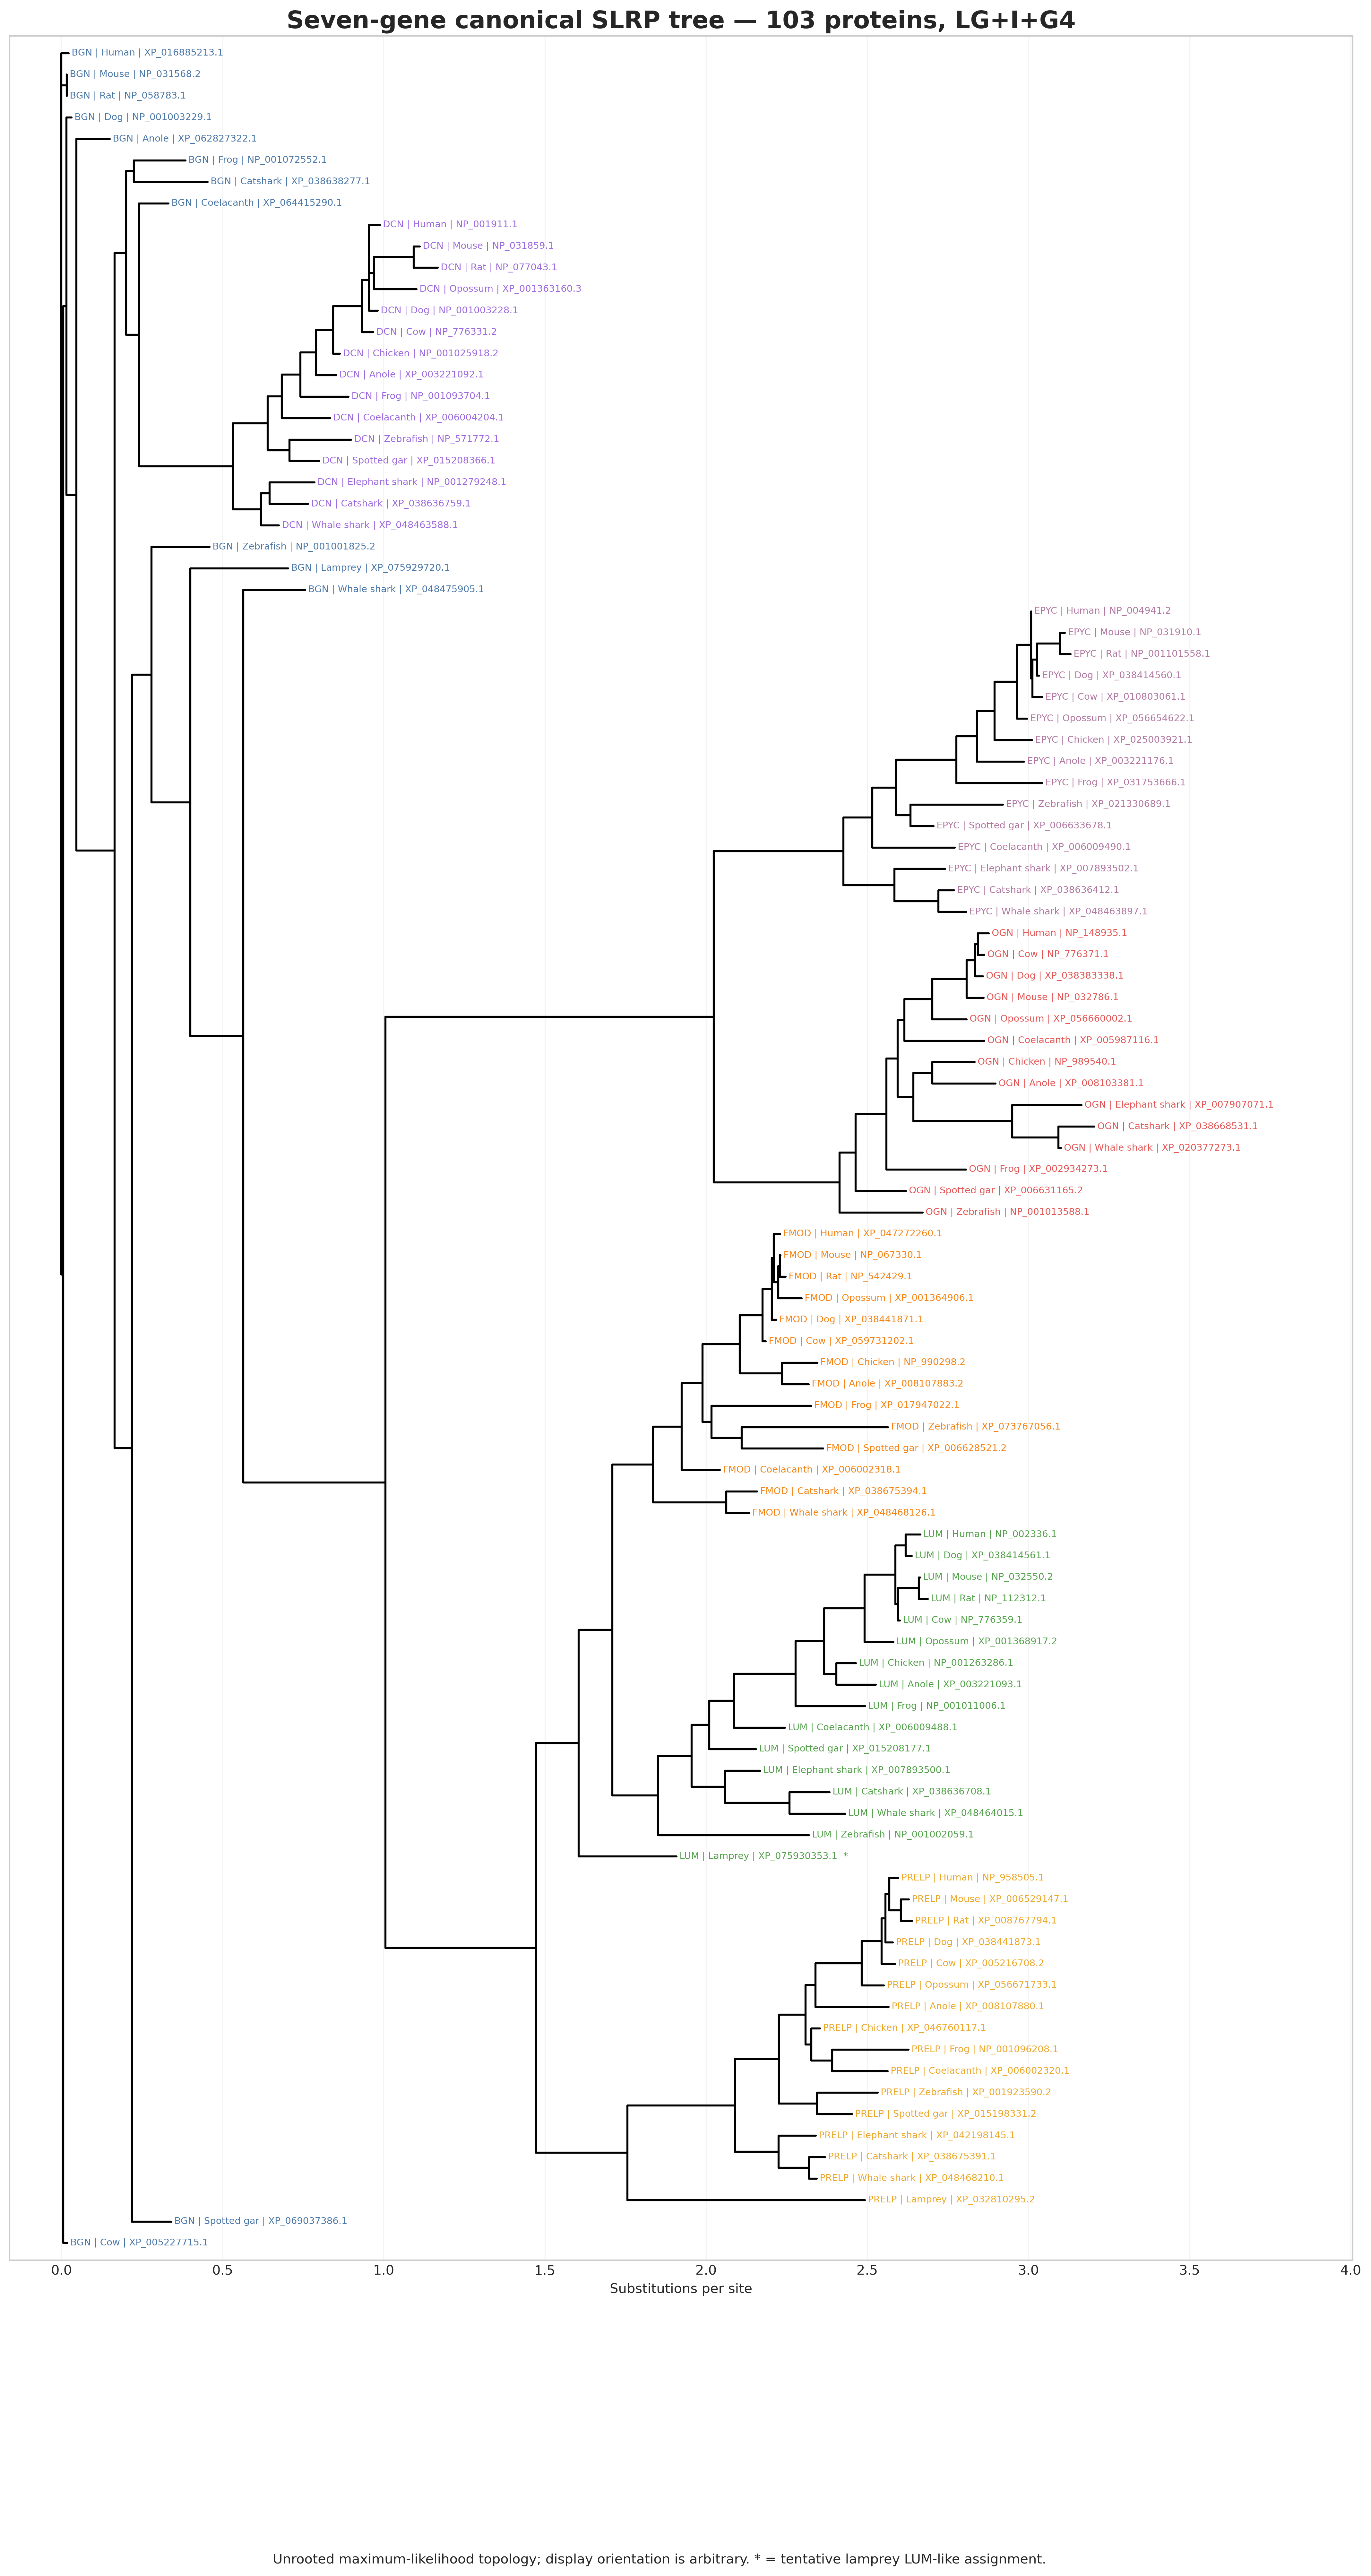
\includegraphics[width=\textwidth,height=0.82\textheight,keepaspectratio]
        {figures/phylogeny/combined_103_protein_tree.png}
    \caption{Unrooted maximum-likelihood phylogeny of the curated 103-protein
    SLRP panel. Tip colours denote the seven gene assignments. DCN, EPYC, FMOD,
    OGN, and PRELP form pure gene-specific unrooted splits; the main LUM split
    contains 15 of 16 sequences, while lamprey LUM is retained tentatively.
    BGN requires the focused BGN/DCN diagnostic rather than interpretation as a
    single pure split. Display orientation does not imply evolutionary
    direction.}
    \label{fig:combined-phylogeny}
\end{figure}

The broader NCBI search was used as a species-expansion analysis rather than as
a replacement for the curated tree. Corrected one-per-locus candidate sets
contained 639 BGN, 632 EPYC, 546 FMOD, 838 LUM, 855 OGN, and 848 PRELP records.
This shows that the workflow can recover homologous candidates far beyond the
15-species panel, but these counts are search outputs rather than verified
ortholog counts. The previously generated large trees were affected by a header-
parsing error that could collapse unrelated loci carrying the same isoform label.
Their topologies are therefore excluded from the thesis evidence. Corrected
large-tree inference remains optional because the curated 103-protein analysis
already answers the principal comparative question.

The targeted species panel provided a separate evolutionary bracket. Amphioxus
did not yield a confident OGN ortholog and instead supplied an informative
SLRP-like uncertainty case. Lamprey retained distinguishable deep-vertebrate
SLRP-like candidates, although the tentative LUM placement showed that closely
related class-II genes remain difficult to resolve at this depth. Cartilaginous-
fish candidates extended recognizable gene-specific architecture to an early
jawed-vertebrate branch but also contained the most obvious partial and
annotation-sensitive BGN/EPYC models. Spotted gar and coelacanth bridged these
deep comparisons to teleosts and tetrapods, allowing teleost divergence or
duplication to be distinguished from loss of ancient vertebrate conservation.
These living species were interpreted as comparative representatives, not as
ancestors of the other sampled lineages.

The species-level summary made this evolutionary pattern quantitative
(Figure~\ref{fig:species-lineage-summary}). Median amino-acid identity to the
human reference was lowest in the three retained lamprey proteins (48.5\%) and
the elephant-shark and catshark sets (51.2\% and 53.2\%), and increased to
85.0--93.5\% in non-human mammals. This trend was not a simple phylogenetic
ladder: spotted gar had a higher median identity (68.1\%) than zebrafish
(61.2\%) or coelacanth (59.8\%). Different gene subsets, lineage-specific rates,
and gene-model quality all contribute to these descriptive medians. Manual
synteny review accepted five of seven loci in both spotted gar and coelacanth,
compared with three of seven in each sampled shark. Amphioxus produced no
accepted gene-specific locus, whereas the seven ambiguous opossum results
reflected incompatible FASTA/GFF inputs rather than evolutionary divergence.

\begin{figure}[tbp]
    \centering
    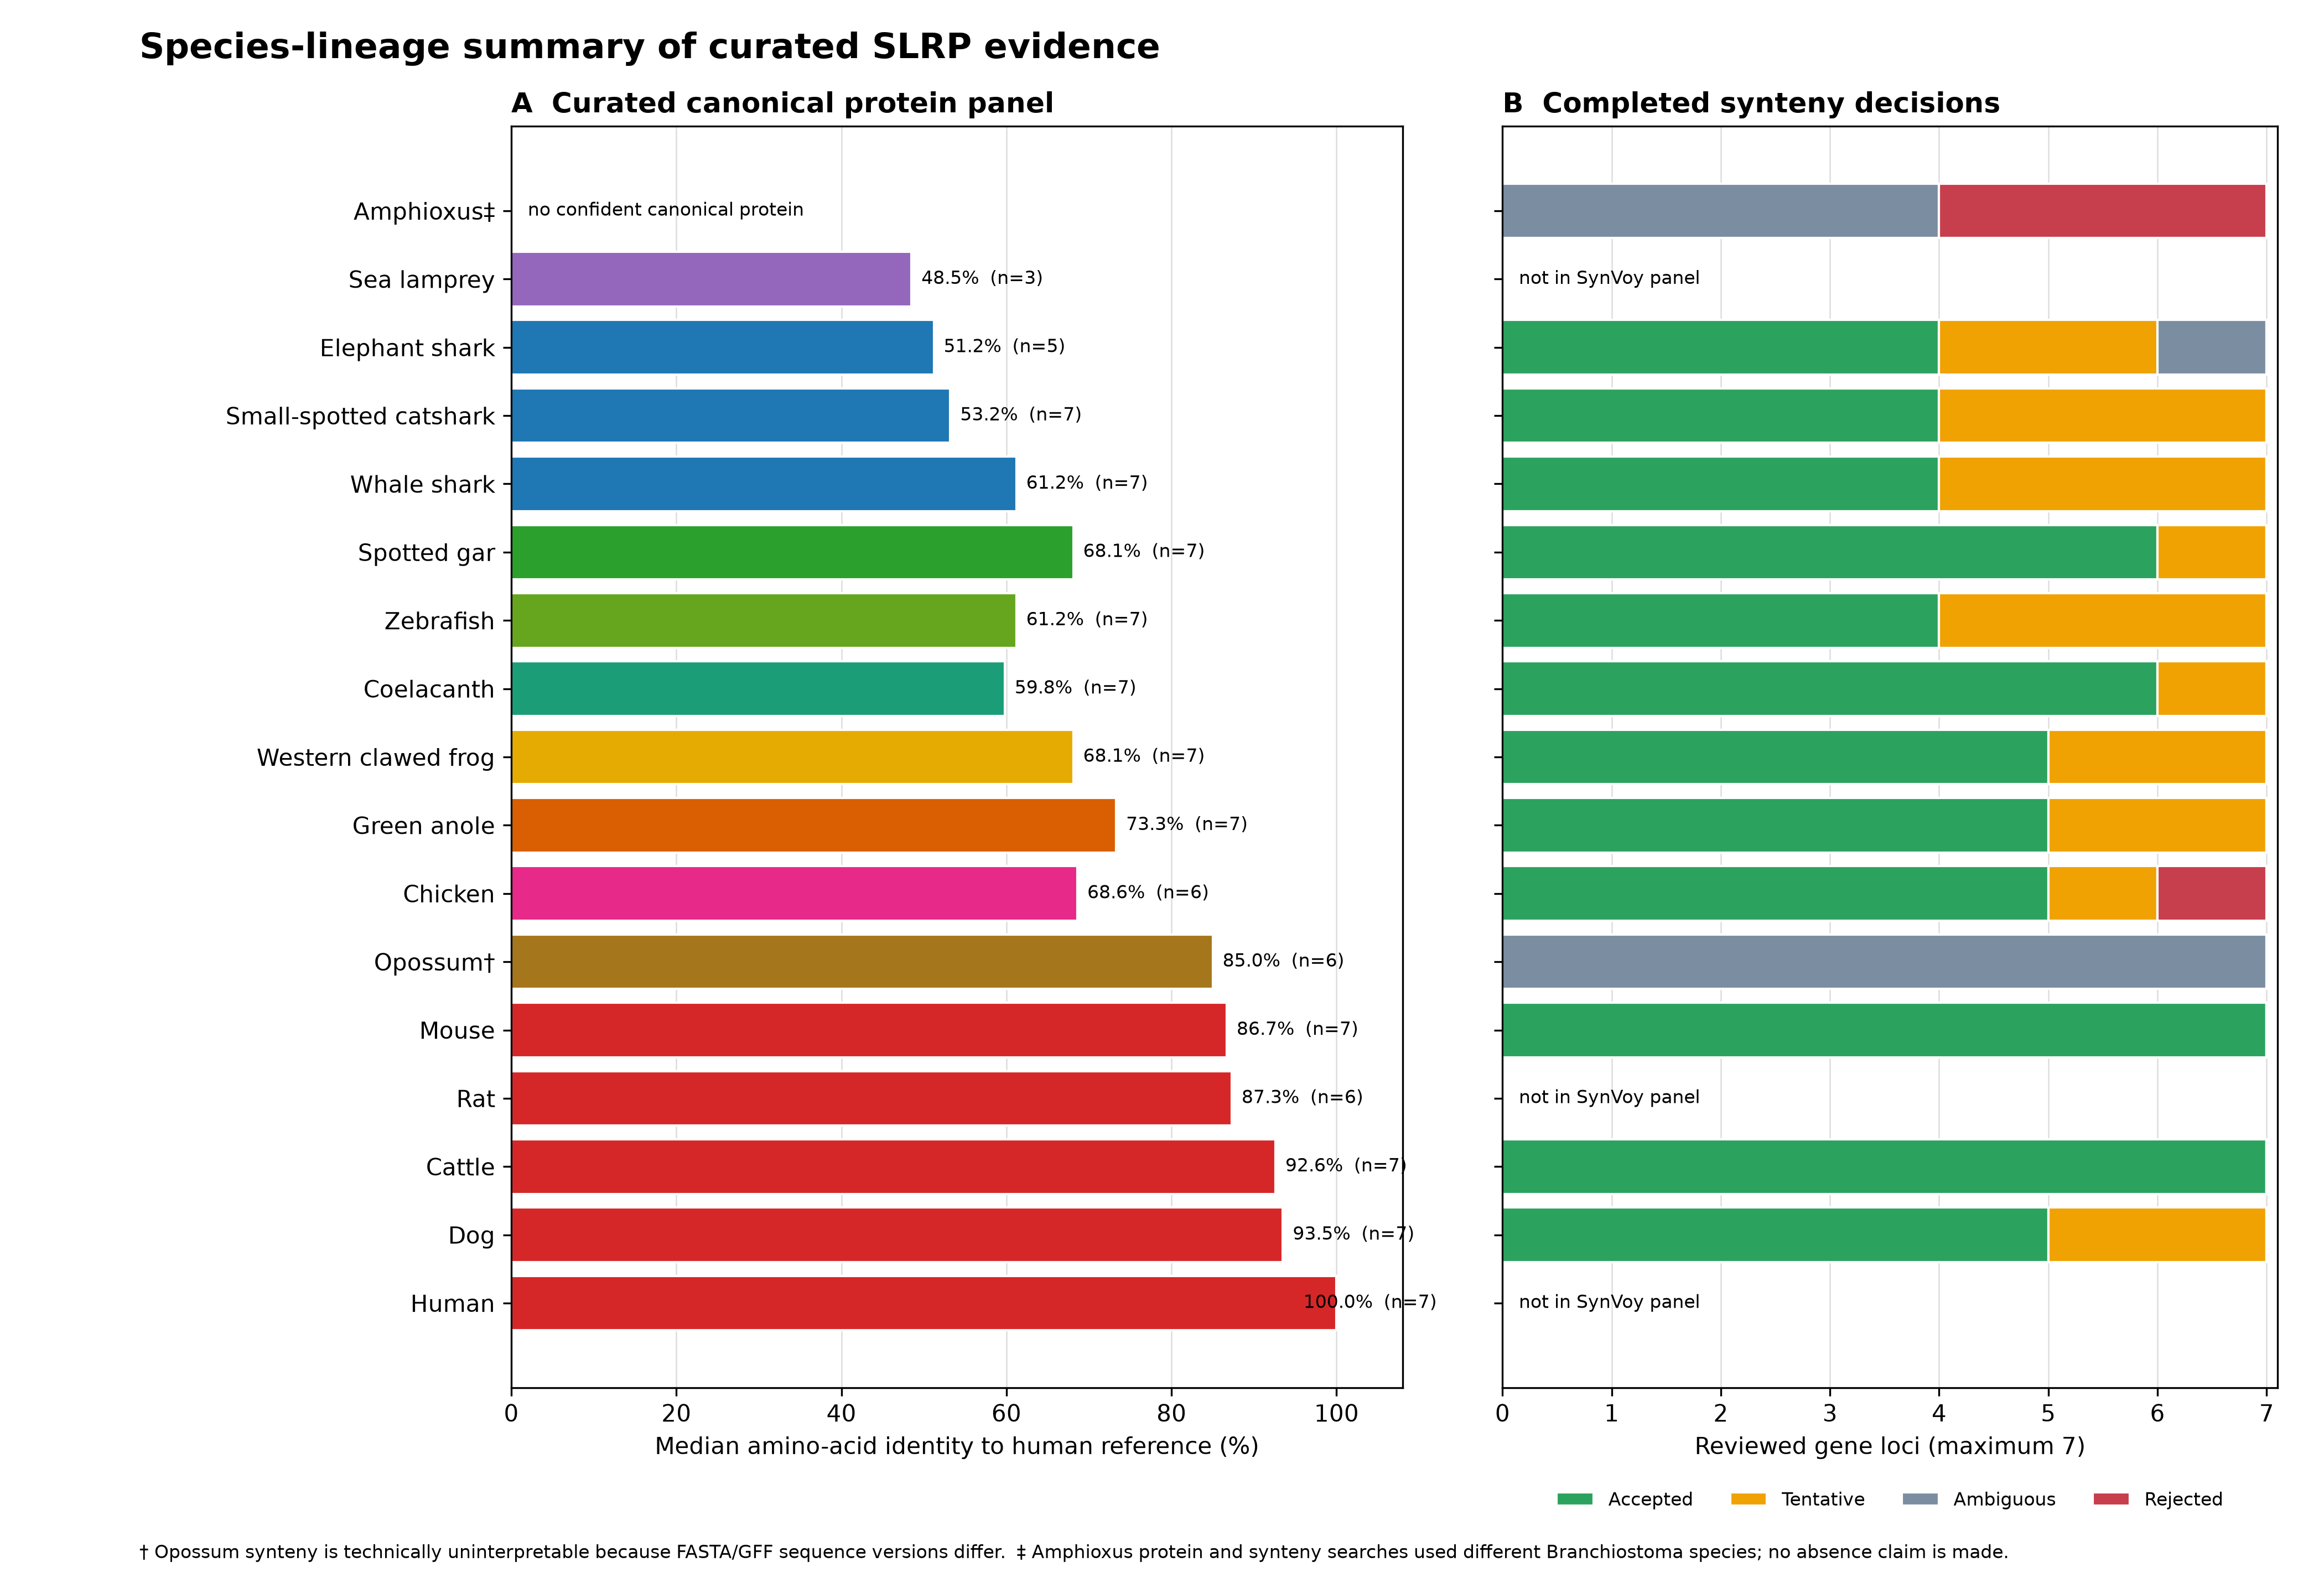
\includegraphics[width=\textwidth]{figures/overview/species_lineage_evidence_summary.png}
    \caption[Species-lineage summary of curated SLRP evidence]{Species-lineage
    summary of the curated comparative evidence. (A) Median amino-acid identity
    to the human reference across the canonical proteins available for each
    species; labels give the number of retained proteins and bar colours denote
    lineage groups. Medians based on different gene subsets are descriptive and
    are not a molecular-clock analysis. (B) Recorded locus-audit decisions
    across the seven focal genes. Rat and lamprey were not SynVoy targets, and
    human supplied the home locus. Opossum calls are technically uninterpretable
    because the FASTA/GFF sequence versions differ. The amphioxus protein and
    synteny searches used different \textit{Branchiostoma} species, and absence
    of a confident candidate was not interpreted as gene loss.}
    \label{fig:species-lineage-summary}
\end{figure}

\subsection{Microsynteny and manual locus-review status}
\label{subsec:results-synteny}

Completed SynVoy reports for BGN, DCN, EPYC, FMOD, LUM, OGN, and PRELP were
parsed across 14 non-human target genomes, yielding a 98-row gene-by-genome
evidence table. The numbers of genomes with a best retained HIGH call were 9
for BGN, 10 for DCN, 9 for EPYC, 10 for FMOD, 10 for LUM, 13 for OGN, and 11
for PRELP. HIGH and MEDIUM values identify retained automated candidates, not
verified one-to-one orthologs, because one genome can contribute multiple calls
or a rescue-derived candidate. The automated results were therefore used to
locate and prioritize loci rather than as a binary orthology test.

The review scheme assigned 26 rows to detailed P1 feature and neighbourhood
inspection, 68 to rapid P2 accession--locus confirmation, and four to P3
controls. All 98 rows have a recorded evidence-based decision: 62 were
accepted, 20 retained as tentative, 12 remained ambiguous, and four were
rejected. These decisions include batch GFF/accession checks and should not be
read as 98 independent visual GDV confirmations. In 69 combinations,
the canonical protein accession directly overlapped the best post-ownership
SynVoy locus in the exact target GFF3, showing that the automated coordinate
and the protein analysed elsewhere represented the same model in those cases.

Detailed review showed why the remaining automated calls could not be read as
a one-to-one orthology table. Canonical EPYC in coelacanth, elephant shark and
spotted gar; LUM in catshark, coelacanth and spotted gar; and PRELP in zebrafish
were accepted using concordant locus, flanking-gene, protein and tree evidence.
The vertebrate \textit{EPYC--KERA--LUM--DCN} region was especially informative:
the corresponding block and several distal anchors remained ordered in
coelacanth, spotted gar and zebrafish even when SynVoy selected a different
fragment. By contrast, the amphioxus EPYC and FMOD intervals overlapped
unrelated RUN-domain- and BRD3-like genes, respectively, and the amphioxus OGN
raw calls were assigned to other genes. Chicken \texttt{XP\_414298.2} was also
rejected from BGN because its product, focused tree and locus neighbours were
ASPN-like.

The locus audit additionally resolved duplicated or annotation-sensitive FMOD
cases. In zebrafish, \textit{fmodb} was the better full-length human-FMOD match,
whereas \textit{fmoda} retained the ancestral FMOD--PRELP neighbourhood; both
were therefore retained as co-ortholog evidence. The updated-tool FMOD report
was integrated rather than treated as a pending rerun. It contained 10 HIGH and
five MEDIUM retained calls, compared with 12 HIGH and seven MEDIUM in the
historical report. Most changes did not alter the final biological decision,
but in spotted gar the updated best HIGH rescue directly overlapped canonical
\textit{fmoda}; eight shared human flanking genes independently supported that
locus. Amphioxus remained rejected, whereas catshark, whale shark, and
zebrafish retained qualified decisions based on the combined locus and protein
evidence rather than the automated rank alone. The elephant-shark
fibromodulin-like model remained
tentative despite a complete 684-aa translation from nine CDS segments. BLASTP
assigned residues 1--330 most strongly to DCN (47.0\% identity) and residues
376--684 most strongly to FMOD (57.0\% identity; 82.2\% coverage of human
FMOD). Pfam detected LRR architecture across both halves and separate LRR
N-terminal caps at residues 54--76 and 383--412. Together with a second
hydrophobic segment at residues 330--347, this supported a compound or fused
gene model rather than a confident single-copy FMOD protein. The locus was
retained as tentative FMOD evidence, but the protein was excluded from the
confident FMOD panel.

All seven opossum rows were classified as ambiguous for synteny because the
GFF3 and FASTA used for those completed reports had incompatible chromosome
sequence versions. A replacement GCF\_027887165.2 pair subsequently passed the
identifier audit, but its gene-level reruns were not complete at the data
freeze. This technical exclusion does not invalidate independently supported
opossum proteins, but it prevents use of the completed SynVoy scores as locus
evidence.
A gene absent from a retained SynVoy call was otherwise recorded as unresolved,
not as a demonstrated evolutionary loss. Figure~\ref{fig:synvoy-overview}
separates the automated call from the recorded integrated locus decision.

\begin{figure}[htbp]
    \centering
    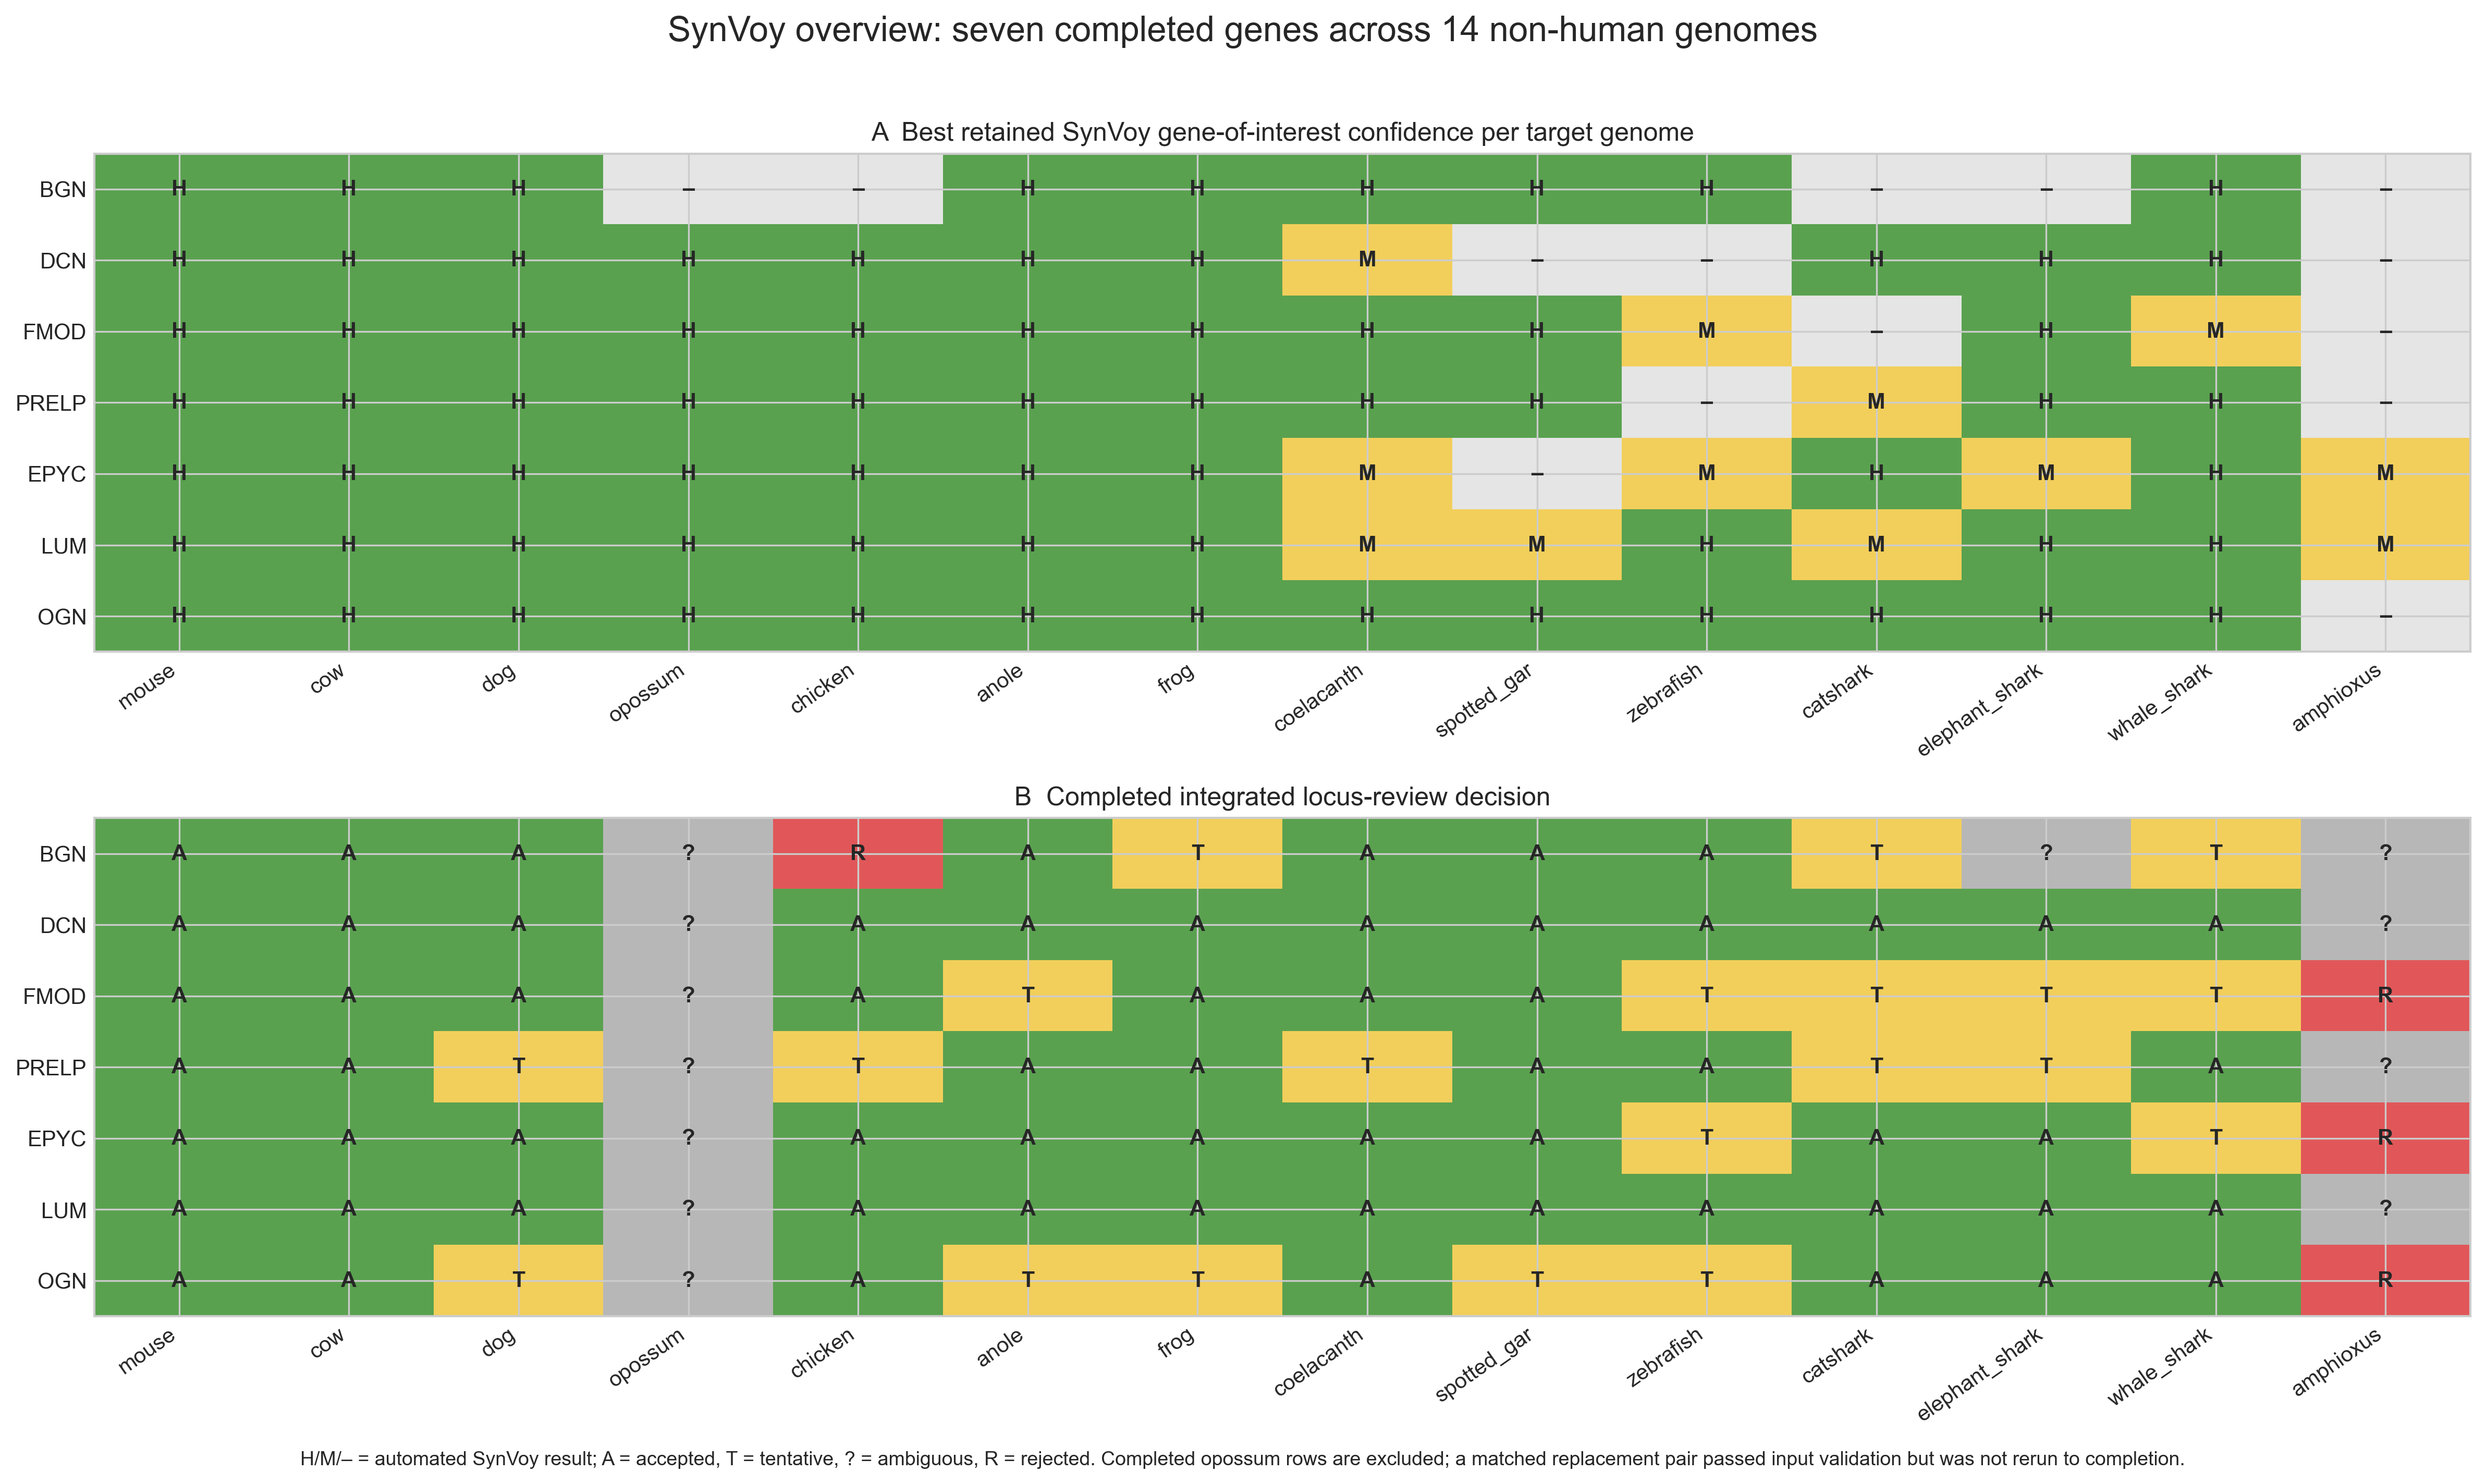
\includegraphics[width=\textwidth,height=0.76\textheight,keepaspectratio]
        {figures/synteny/synvoy_species_confidence_heatmap.png}
    \caption{SynVoy locus-level evidence and recorded review outcomes for seven
    genes across 14 non-human target genomes. Panel A shows the best retained
    automated candidate class after ownership/paralog filtering: H, HIGH; M,
    MEDIUM; dash, no retained HIGH/MEDIUM call. Panel B shows the integrated
    locus decision: A, accepted; T, tentative; question mark, ambiguous; R,
    rejected. Decisions combine exact-assembly GFF/accession checks with
    detailed review of prioritized exceptions; they are not 98 independent
    visual GDV confirmations. A missing automated call is not evidence of gene loss. All
    opossum outcomes are ambiguous because the target FASTA and GFF3 sequence
    identifiers were incompatible.}
    \label{fig:synvoy-overview}
\end{figure}

\subsection{Conserved coding organization and domain--exon architecture}
\label{subsec:results-gene-structure}

Representative protein-coding transcripts were compared for human, mouse, cow,
chicken, and zebrafish. Coding-exon number was constant across the five species
for each examined gene: seven CDS exons for BGN and DCN, six for EPYC and OGN, and two
for FMOD, PRELP, LUM, and OMD. Estimated protein lengths were correspondingly
stable, whereas total gene span varied more strongly because of intron-length
differences. No representative transcript was flagged as a structural outlier.
All 40 selected annotation models produced genome-reconstructed CDSs that were
divisible by three, began with methionine, contained a terminal stop codon, and
lacked internal stops; all coding blocks also passed their GFF phase-continuity
checks. These are annotation-quality results rather than automatic orthology
validation. The accession crosswalk identified 18 exact canonical-panel
accessions and 15 alternative accessions with equivalent or near-equivalent
translations. Zebrafish BGN structure was represented by \textit{bgna}, whereas
the canonical protein panel used \textit{bgnb}. The technically complete chicken
BGN-locus transcript encoded the ASPN-like product \texttt{XP\_414298.2} and was
therefore not counted as independent BGN orthology support. OMD remained a
five-species context-only comparison.

The higher-resolution splice analysis identified 26 coding junctions that were
comparable across all five species. Intron phase was conserved for all 26.
Exact boundary positions were especially close for BGN, for which all six
junctions varied by at most three amino acids, and for the single OMD junction,
which varied by two amino acids. The remaining genes preserved phase despite
modest boundary displacement (median gene-level ranges of 6--18 amino acids).
Thus, the shared exon counts represent a conserved frame-compatible coding
organization rather than only the same number of annotated boxes.
For BGN, this statement describes the selected annotated BGN-like/co-ortholog
set and does not override the chicken product conflict or the zebrafish
\textit{bgna}/\textit{bgnb} distinction.

The annotation-level isoform screen identified coding alternatives that could
change CDS-exon count and/or protein length at 11 of 40 loci. These flags were
concentrated in BGN (mouse and zebrafish), FMOD (zebrafish), PRELP (chicken),
EPYC (human, chicken, and zebrafish), LUM (cow), and OGN (human and zebrafish).
They identify transcript-choice sensitivity rather than representative-model
failure; all selected models passed the sequence-completeness checks. Full UTR
lengths varied much more than the coding organization and were therefore kept
as annotation-sensitive descriptive data. This conserved coding organization
supported stable gene models, but was interpreted together with protein, tree,
domain, and locus evidence rather than as stand-alone proof of orthology.

The representative-protein Pfam rescan recovered significant LRR-family
support in all 40 translations (294 significant repeat/domain hits in total).
At least one LRR-family model crossed a coding-exon boundary in representatives
of BGN, FMOD, PRELP, EPYC, LUM, and OGN; OMD hits remained within one coding
exon. The human domain--exon map therefore shows that the LRR-rich architecture
is generally distributed across the conserved coding framework rather than
being encoded as one independent exon-level module. The cross-species overview
in Figure~\ref{fig:gene-structure-overview} focuses on conserved coding
organization and distinguishes it from more variable total gene span.

\begin{figure}[p]
    \centering
    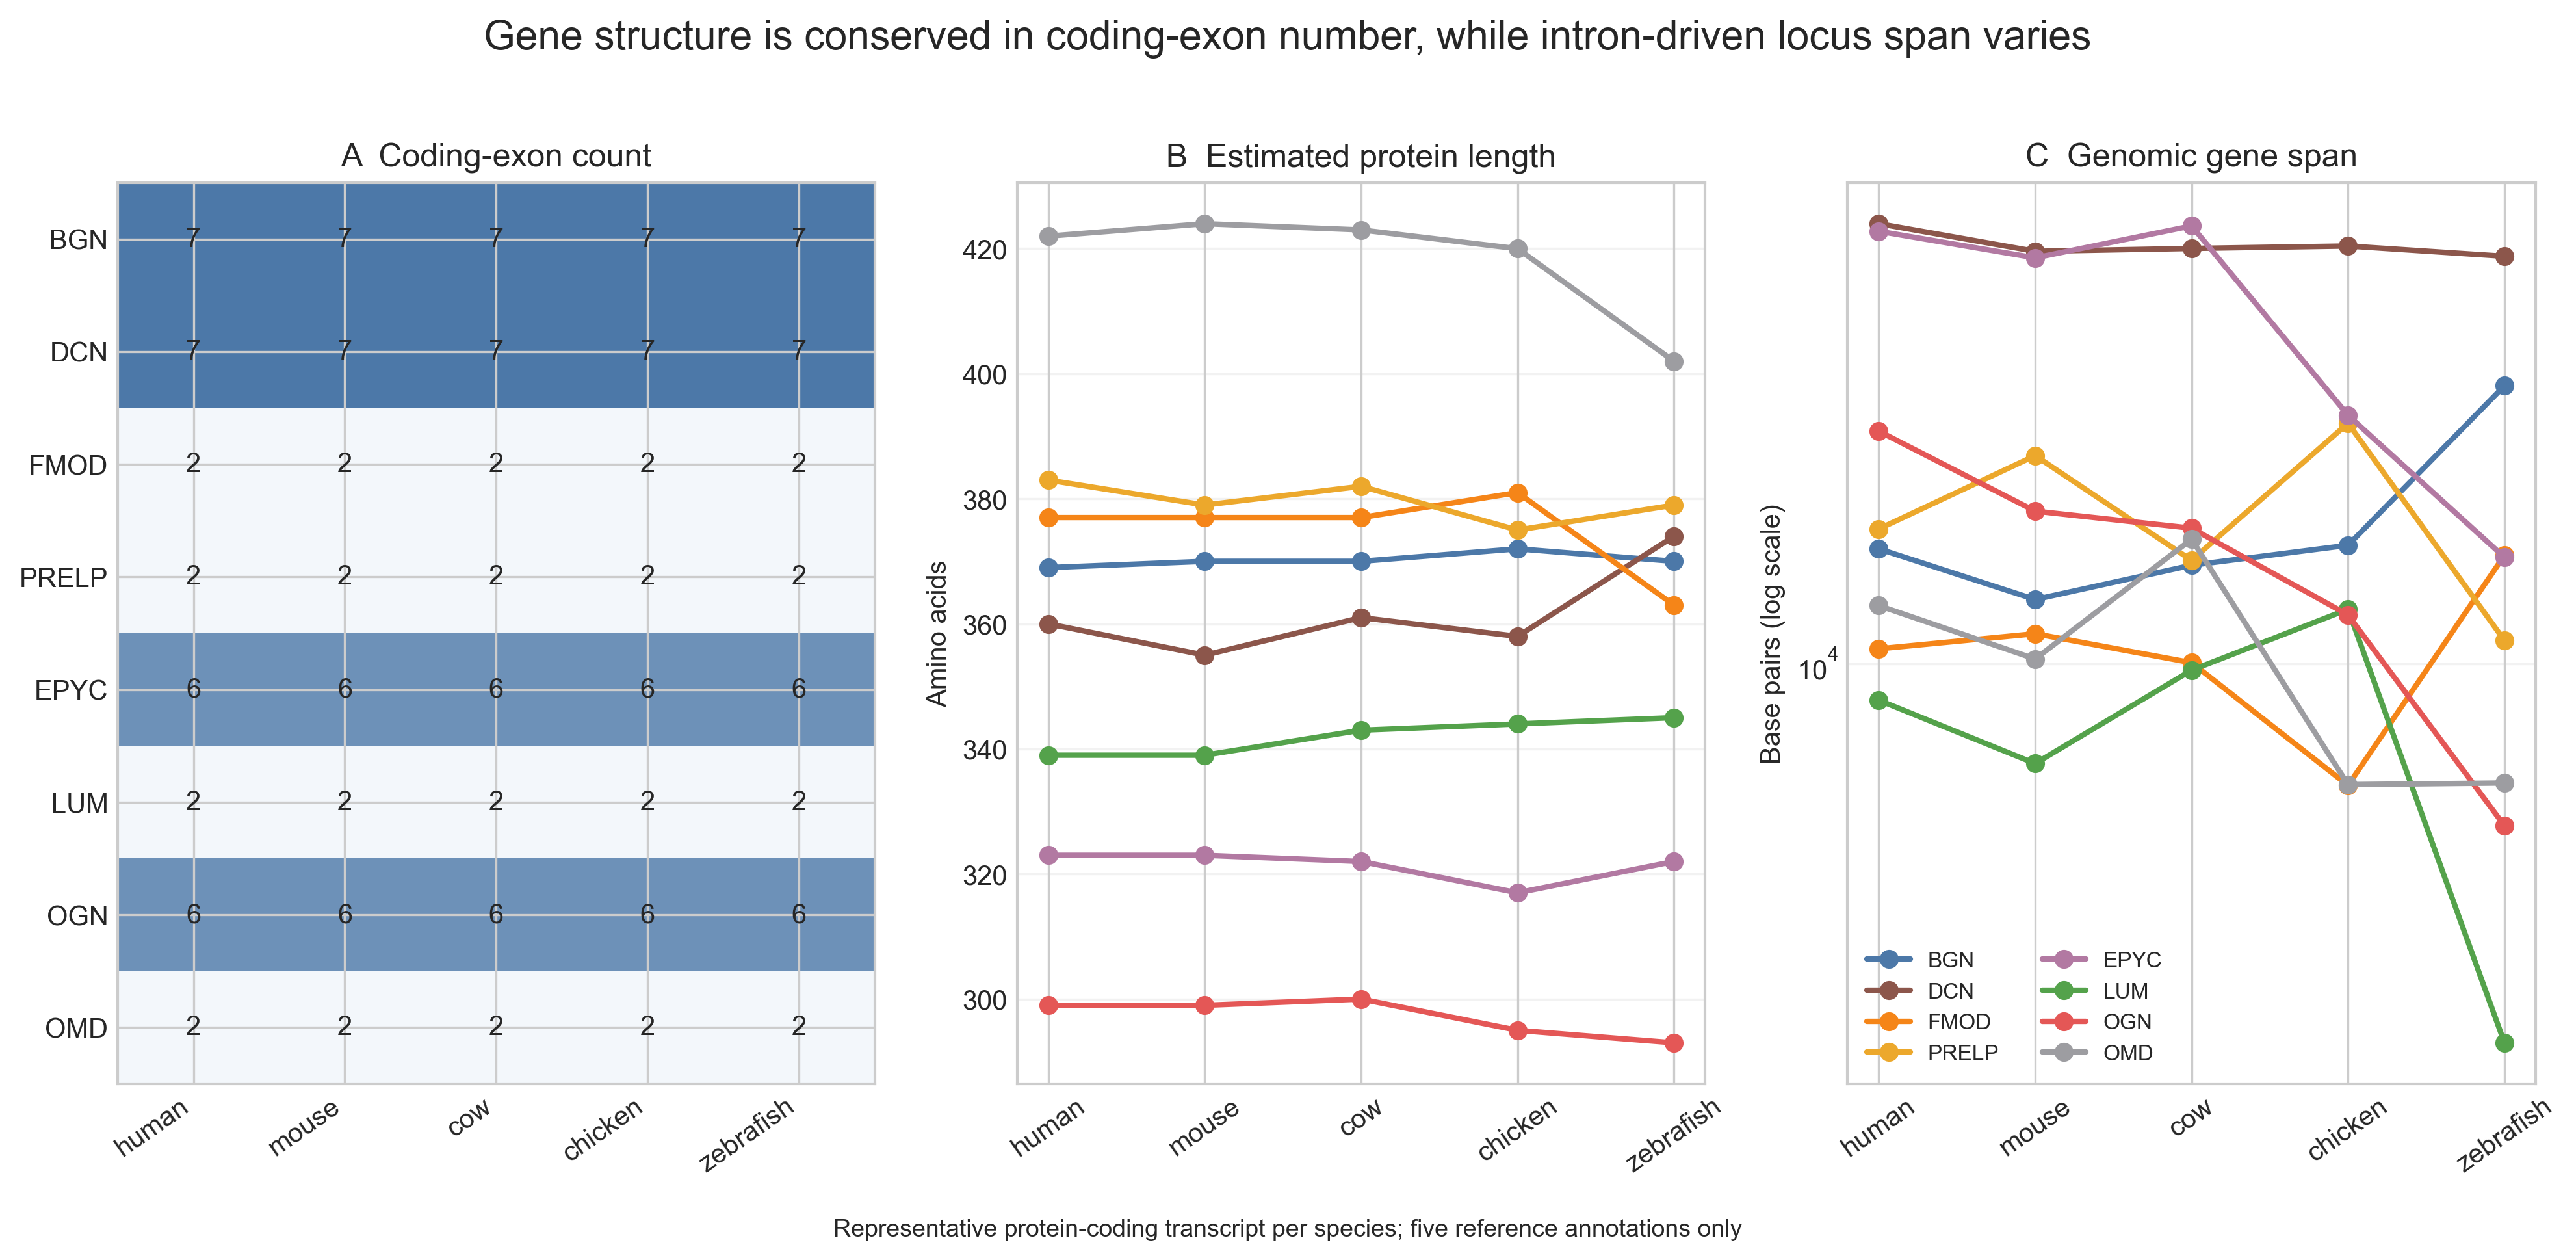
\includegraphics[width=\textwidth,height=0.82\textheight,keepaspectratio]
        {figures/gene_structure/gene_structure_conservation_overview.png}
    \caption{Conservation of representative protein-coding gene structure in
    human, mouse, cow, chicken, and zebrafish. Coding-exon number is stable
    within each of the seven comparative genes and OMD context, and estimated
    protein length is much more stable than intron-dependent genomic span.
    Results depend on the selected representative annotation and support gene-
    model plausibility rather than orthology by themselves. The chicken BGN
    annotation is structurally coherent but its product is ASPN-like, and the
    zebrafish BGN structure row represents \textit{bgna} rather than the
    canonical-panel \textit{bgnb}.}
    \label{fig:gene-structure-overview}
\end{figure}

\subsection{Supplementary coding-sequence constraint}
\label{subsec:results-codon-constraint}

Twenty-five of the 32 possible human--target NG86 comparisons produced a finite
$d_N/d_S$ estimate after excluding the ASPN-like chicken BGN-locus product.
Every interpretable ratio was below one (range 0.031--0.240), consistent with
predominant purifying constraint on these representative coding sequences.
Six human--zebrafish comparisons had undefined or non-positive $d_S$
and were not interpreted; PRELP was the exception ($d_N/d_S=0.203$).
Human--chicken EPYC and LUM also remained below one but had $d_S>2$ and were
flagged for possible synonymous-site saturation. The analysis therefore adds a
nucleotide-level constraint check for shallow and moderate comparisons, while
deep vertebrate comparisons remain outside its reliable range.

\subsection{Curated mouse and human phenotype evidence}
\label{subsec:results-phenotypes}

The MGI analysis recovered 118 focal records and 105 unique
gene--Mammalian-Phenotype-term--evidence combinations; all recovered focal
records represented single-gene genotypes in the downloaded release. BGN had
19 unique phenotype terms, including 14 skeletal/cartilage/joint terms; DCN had
24 terms, including 4 in that category; FMOD had
8 terms, including 4 in that category; and EPYC had 3 terms, including short
femur and osteoarthritis. LUM had 31 terms dominated by corneal and
skin/connective-tissue phenotypes, with one tendon-related skeletal term. OGN
had 8 terms dominated by corneal, collagen/skin, cardiovascular, and metabolic
annotations. PRELP had 12 terms but no term assigned to the broad
skeletal/cartilage/joint category in this release.

The pinned HPO release contained 89 focal gene--phenotype rows: 79 for BGN and
10 for DCN. It linked BGN to Mendelian OMIM:300106 and OMIM:300989 and DCN to
OMIM:610048. The absence of HPO rows for the other five genes was treated as a lack of curated human
disease annotation in that release, not as evidence of absent biological
function. Because phenotype-database counts depend on study and curation depth,
they were not used to rank candidate importance.

\subsection{Supplementary mature-protein motif analysis}
\label{subsec:results-protein-motifs}

MEME identified recurrent sequence blocks in the mature-protein proxies: 37
motifs in the combined 103-protein panel and 79 motifs across the seven separate
gene models; STREME returned 35 gene-enriched patterns. Signal peptides were
removed from all 100 SignalP-positive proteins, whereas the three
SignalP-negative proteins remained untrimmed. The motifs were dominated by
conserved LRR-rich and
cysteine-rich sequence blocks and were therefore interpreted as sequence
conservation rather than as experimentally established functional sites.

When every protein was scanned against all seven gene-specific motif models,
all 103 proteins scored most strongly against the model learned from their
assigned gene. Thus, the motif analysis supplied no new candidate outlier. It
added classification support to the curated assignments but did not remove
independent reciprocal-hit, coverage, partial-model, or SignalP caveats. Because
the same small curated sets were used to learn and evaluate the models and no
independent hold-out was available, this was not treated as an independent
accuracy estimate.

\subsection{Supplementary exploratory promoter analysis}
\label{subsec:results-promoter-motifs}

Seventy strand-aware promoter sequences were extracted from 35 representative
loci: core and proximal windows for each of seven genes in human, mouse, cow,
chicken, and zebrafish. All sequences had their expected length, none was
clipped at a contig edge, and none contained ambiguous bases. Proximal-promoter
GC content ranged from 32.48\% to 59.06\%.

No site from the targeted 40-profile transcription-factor panel passed the
strict FIMO threshold of $q\leq0.05$, and no targeted motif reached the
panel-corrected AME threshold of $E<0.05$. HIF1A was the strongest targeted AME
result (raw $p=7.49\times10^{-5}$; within-motif adjusted $p=0.0638$), but its
panel-corrected E-value was 2.55. Twelve motifs from the full JASPAR collection
passed $E<0.05$; several were A-rich, T-rich, or repetitive, as were many global
de-novo motifs. The analysis therefore did not identify a statistically
supported shared cartilage/growth-plate regulatory signature. Uncorrected
cross-species recurrences were retained only as hypotheses for future
chromatin-occupancy or reporter experiments.

\subsection{Integrated gene-level interpretation}
\label{subsec:results-gene-specific-summary}

BGN and FMOD provided the strongest combined expression and technical anchors.
DCN contributed direct cartilage/ECM support and the essential class-I paralog
control that exposed contaminated BGN assignments.
PRELP was strongly supported by the direct zone-resolved growth-plate dataset
despite only moderate abundance in the broader P0 lineage sample. EPYC had lower
RNA abundance but a direct anatomical rationale and coherent comparative
evidence. LUM had a clean protein and gene-structure profile; manual locus
review accepted its canonical catshark, coelacanth, and spotted-gar loci despite
different SynVoy-selected fragments, while amphioxus remained unresolved. OGN contributed evolutionary and
class-III breadth but remained the least certain growth-plate candidate; its
final vertebrate set was coherent only after exclusion of the amphioxus
SLRP-like sequence and tentative treatment of spotted gar.
Figure~\ref{fig:integrated-evidence} places these gene-level findings side by
side while preserving the original units and caveats of each evidence layer.

\begin{figure}[p]
    \centering
    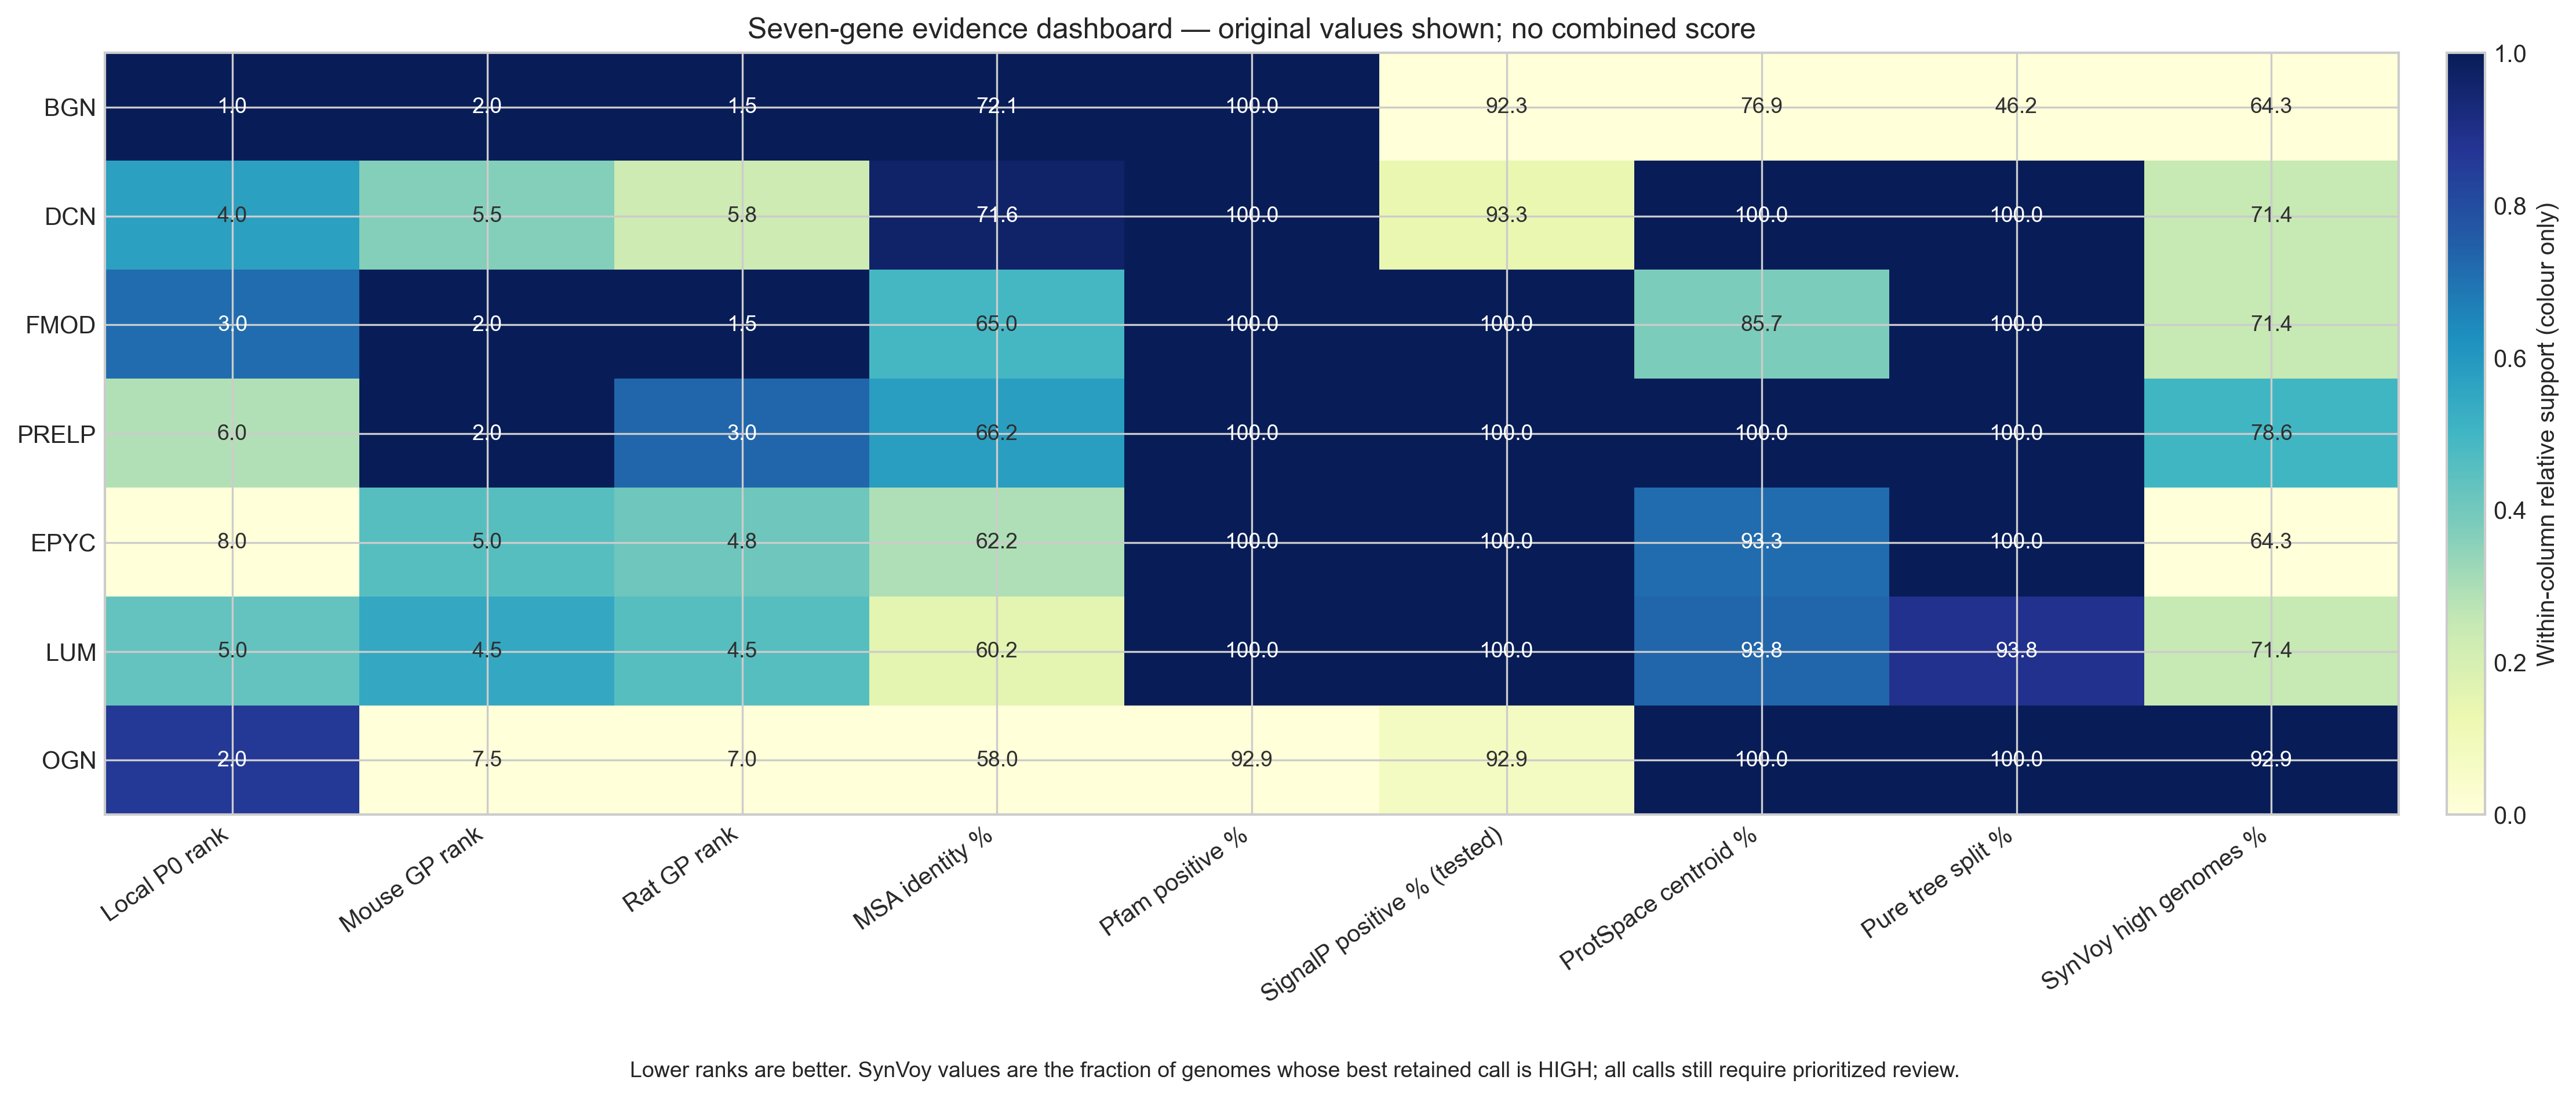
\includegraphics[width=\textwidth,height=0.82\textheight,keepaspectratio]
        {figures/overview/integrated_evidence_dashboard.png}
    \caption{Integrated evidence summary for the seven-gene comparative panel.
    Expression, protein/domain, phylogenetic, synteny, gene-structure, motif,
    and phenotype evidence retain their original units and limitations; panel
    colours are normalized within evidence types and are not combined into an
    unsupported numerical confidence score.}
    \label{fig:integrated-evidence}
\end{figure}
